%% fcup-thesis.tex -- document template for PhD theses at FCUP
%%
%% Copyright (c) 2015 João Faria <joao.faria@astro.up.pt>
%%
%% This work may be distributed and/or modified under the conditions of
%% the LaTeX Project Public License, either version 1.3c of this license
%% or (at your option) any later version.
%% The latest version of this license is in
%%     http://www.latex-project.org/lppl.txt
%% and version 1.3c or later is part of all distributions of LaTeX
%% version 2005/12/01 or later.
%%
%% This work has the LPPL maintenance status "maintained".
%%
%% The Current Maintainer of this work is
%% João Faria <joao.faria@astro.up.pt>.
%%
%% This work consists of the files listed in the accompanying README.

%% SUMMARY OF FEATURES:
%%
%% All environments, commands, and options provided by the `ut-thesis'
%% class will be described below, at the point where they should appear
%% in the document.  See the file `ut-thesis.cls' for more details.
%%
%% To explicitly set the pagestyle of any blank page inserted with
%% \cleardoublepage, use one of \clearemptydoublepage,
%% \clearplaindoublepage, \clearthesisdoublepage, or
%% \clearstandarddoublepage (to use the style currently in effect).
%%
%% For single-spaced quotes or quotations, use the `longquote' and
%% `longquotation' environments.


%%%%%%%%%%%%         PREAMBLE         %%%%%%%%%%%%

%%  - Default settings format a final copy (single-sided, normal
%%    margins, one-and-a-half-spaced with single-spaced notes).
%%  - For a rough copy (double-sided, normal margins, double-spaced,
%%    with the word "DRAFT" printed at each corner of every page), use
%%    the `draft' option.
%%  - The default global line spacing can be changed with one of the
%%    options `singlespaced', `onehalfspaced', or `doublespaced'.
%%  - Footnotes and marginal notes are all single-spaced by default, but
%%    can be made to have the same spacing as the rest of the document
%%    by using the option `standardspacednotes'.
%%  - The size of the margins can be changed with one of the options:
%%     . `narrowmargins' (1 1/4" left, 3/4" others),
%%     . `normalmargins' (1 1/4" left, 1" others),
%%     . `widemargins' (1 1/4" all),
%%     . `extrawidemargins' (1 1/2" all).
%%  - The pagestyle of "cleared" pages (empty pages inserted in
%%    two-sided documents to put the next page on the right-hand side)
%%    can be set with one of the options `cleardoublepagestyleempty',
%%    `cleardoublepagestyleplain', or `cleardoublepagestylestandard'.
%%  - Any other standard option for the `report' document arclass can be
%%    used to override the default or draft settings (such as `10pt',
%%    `11pt', `12pt'), and standard LaTeX packages can be used to
%%    further customize the layout and/or formatting of the document.

%% *** Add any desired options. ***
%PDF
%\documentclass[a4paper,narrowmargins,11pt,oneside,draft,onehalfspaced,singlespacednotes]{fcup-thesis}
%\documentclass[a4paper,narrowmargins,11pt,oneside,onehalfspaced,singlespacednotes]{fcup-thesis}
%Print
%\documentclass[draft,a4paper,narrowmargins,11pt,twoside,openright,onehalfspaced,singlespacednotes]{fcup-thesis}
\documentclass[a4paper,narrowmargins,11pt,twoside,openright,onehalfspaced,singlespacednotes]{fcup-thesis}

%% *** Add \usepackage declarations here. ***
%% The standard packages `geometry' and `setspace' are already loaded by
%% `ut-thesis' -- see their documentation for details of the features
%% they provide.  In particular, you may use the \geometry command here
%% to adjust the margins if none of the ut-thesis options are suitable
%% (see the `geometry' package for details).  You may also use the
%% \setstretch command to set the line spacing to a value other than
%% single, one-and-a-half, or double spaced (see the `setspace' package
%% for details).


%%%%%%%%%%%%%%%%%%%%%%%%%%%
% Overfull statements fix %
%%%%%%%%%%%%%%%%%%%%%%%%%%%
\pretolerance=150
\setlength{\emergencystretch}{3em}

%%%%%%%%%%%%%%%%%%%%%%%%%%
% Standard british babel %
%%%%%%%%%%%%%%%%%%%%%%%%%%
\usepackage[english]{babel}

% Enable array for text formatting 
\usepackage{array}

% Standard Mathematics library 
\usepackage{amsmath}  

% Standard symbols for asmath library
\usepackage{amssymb}

%%%%%%%%%%%%%%%%%%%%%%%%%%%%%%%%%%%%%%%%%%%
% Override the basic math font with arial %
%%%%%%%%%%%%%%%%%%%%%%%%%%%%%%%%%%%%%%%%%%%
% Math font specification package
\usepackage{mathspec}

% Proporitional lining for digits latin and greek letters
\setmathsfont(Digits)[Numbers={Lining,Proportional}]{Arial}
\setmathsfont(Latin)[Numbers={Lining,Proportional}]{Arial}
\setmathsfont(Greek)[Numbers={Lining,Proportional}]{Arial}

% Main direction symbols for integrals derivations etc
\usepackage{mdsymbol}

% asmath symbols and additional library
\usepackage{amsthm}      

% Enable usage of Eulerscript for special math symbols
\usepackage[mathscr]{euscript}

%%%%%%%%%%%%%%
% Algorithms %
%%%%%%%%%%%%%%
% Enable algorithms - nice format use chapter numbering
\usepackage[ruled,algochapter]{algorithm2e}

% custom keywords for alggorithms
\usepackage{algorithmic}

%%%%%%%%
% Misc %
%%%%%%%%
% Enable bold symbols in math mode (unused ?)
\usepackage{bm}

% Enhanced support for graphics (ugly hack on big schemes)
\usepackage{graphicx}       

% Replace strings in encapsulated PostScript figures (Arial to my PS files ...)
\usepackage{psfrag}         

% Sophisticated verbatim text (nice notes and foootnotes)
\usepackage{fancyvrb}    

%Im­proves the in­ter­face for defin­ing float­ing ob­jects such as fig­ures and ta­bles. In­tro­duces the boxed float, the ruled float and the plain­top float. You can de­fine your own floats and im­prove the be­haviour of the old ones.  The pack­age also pro­vides the H float mod­i­fier op­tion of the ob­so­lete here pack­age. You can se­lect this as au­to­matic de­fault with \float­place­ment{fig­ure}{H}. (Nice floats and fixed figures/algorithms/equations).
\usepackage{float}

%Mod­i­fies the tab­u­larx en­vi­ron­ment to com­bine the fea­tures of the tab­u­larx pack­age (auto-sized columns in a fixed width ta­ble) with those of the longtable pack­age (multi-page ta­bles). 
\usepackage{ltablex}

%Library bibtex wrapper, square brackets, sort by first author surname, use coma seprarator, use number labeling
\usepackage[square,sort,comma,numbers]{natbib}        

%A sym­bol font (dis­tributed as METAFONT source) that con­tains many of the sym­bols of the Zapf ding­bats set, to­gether with an NFSS in­ter­face for us­ing the font.
\usepackage{bbding}

%The dcol­umn pack­age makes use of the ar­ray pack­age to de­fine a "D" col­umn for­mat for use in tab­u­lar en­vi­ron­ments. (Multicollumn enviroment , layered tables)
\usepackage{dcolumn}        

%The pack­age en­hances the qual­ity of ta­bles in LATEX, pro­vid­ing ex­tra com­mands as well as be­hind-the-scenes op­ti­mi­sa­tion. Guide­lines are given as to what con­sti­tutes a good ta­ble in this con­text. From ver­sion 1.61, the pack­age of­fers longtable com­pat­i­bil­ity. (Yet another table hacks)
\usepackage{booktabs} 

%The pack­age has a lot of flex­i­bil­ity, in­clud­ing an op­tion for spec­i­fy­ing an en­try at the “nat­u­ral” width of its text. (Multirow cells in table headres)
\usepackage{multirow}

%Pro­vides enu­mer­ate and item­ize en­vi­ron­ments that can be used within para­graphs to for­mat the items ei­ther as run­ning text or as sep­a­rate para­graphs with a pre­ced­ing num­ber or sym­bol. (Nice paragraph/itemize/enumerate) package
\usepackage{paralist}     

%Draft only enviromental enabler (Deprecated - for table debug mainly)
\usepackage{ifdraft}  

% indentfirst – Indent first paragraph after section header by default disabled 
%\usepackage{indentfirst}    

% Add bibliography/index/contents to Table of Contents (\bibliography{*} command)
\usepackage[nottoc,notlof,notlot]{tocbibind}

% Pretty and clickable urls in 
\usepackage{url}

% multiline collumn tables (Nomenclature)
\usepackage{tabularx}

%%%%%%%%%%%%%%%%%%%%%%%%%%%%%%%%%%%
% Table figure caption subcaption %
%%%%%%%%%%%%%%%%%%%%%%%%%%%%%%%%%%%
% use font size for captions like 8pt -> normalisize 11pt, scriptsize->8pt
\usepackage[font={scriptsize}]{caption}

% use font size for captions like 8pt -> normalisize 11pt, scriptsize->8pt
\usepackage[font={scriptsize}]{subcaption}

% Other packages caption setup, just for ensurance
\captionsetup{font=scriptsize}

% Hypper references - clickable labels 
\usepackage[unicode]{hyperref}

% Specific color package - color by name hex, cmyk etc.
\usepackage{xcolor}

%%%%%%%%%%%%%%%%%%%%%%%%%%%%%%%%%%
% Document setup for referencing %
%%%%%%%%%%%%%%%%%%%%%%%%%%%%%%%%%%
\hypersetup{pdftitle=Obstacle Avoidance Framework based on Reach Sets, 
            pdfauthor=Alojz Gomola,
            colorlinks=false,
            urlcolor=blue,
            pdfstartview=FitH,
            pdfpagemode=UseOutlines,
            pdfnewwindow,
            breaklinks
          }
%%%%%%%%%%%%%%%%%%%%%%          
%% Arrays in tables %%
%%%%%%%%%%%%%%%%%%%%%%       
% Array package import
\usepackage{array}

% Left alignement
\newcolumntype{L}[1]{>{\raggedright\let\newline\\\arraybackslash\hspace{0pt}}m{#1}}

% Center alignement
\newcolumntype{C}[1]{>{\centering\let\newline\\\arraybackslash\hspace{0pt}}m{#1}}

% Right alignement
\newcolumntype{R}[1]{>{\raggedleft\let\newline\\\arraybackslash\hspace{0pt}}m{#1}}         

% Multiline column with text filling
\newcolumntype{B}{X}

% Multiline column with X percentage of text width
\newcolumntype{S}[1]{>{\hsize=#1\textwidth}X}

% twoline cell definition macro
\newcommand{\twolinecellr}[2][r]{%
  \begin{tabular}[#1]{@{}r@{}}#2\end{tabular}}

% Section state macro - deprecated used during writting of thesis
\newcommand{\secState}[1]{
	\ifdraft{(#1) }{}
}

%%%%%%%%%%%%%%%%%%%%
% Figure directory %
%%%%%%%%%%%%%%%%%%%%
\newcommand{\FIGDIR}{./Pics}    %%% directory containing figures

%%%%%%%%%%%%%%%%%%%%%%%%%%%%%%%%%%%%%%%%%%%%%%%%
% Theorems/defs and other structured referables%
%%%%%%%%%%%%%%%%%%%%%%%%%%%%%%%%%%%%%%%%%%%%%%%%
% Plain style of theorems - inline in text
\theoremstyle{plain}

% Theorem keyword definition
\newtheorem{theorem}{Theorem}

% Lemma for theorem keyword definition
\newtheorem{lemma}[theorem]{Lemma}

% Proposition for theorem keyword definition 
\newtheorem{proposition}[theorem]{Proposition}

% If different theorem type for proof/problem/definition is required
\theoremstyle{plain}

% Definition keyword
\newtheorem{definition}{Definition}

% Problem keyword
\newtheorem{problem}{Problem}

% Example keyword
\newtheorem{example}{Example}

% Assumnption keyword
\newtheorem{assumption}{Assumption}

% Remark style without numbering
\theoremstyle{remark}

% Corollary keyword definition
\newtheorem*{corollary}{Corollary}
% Note keyword definition
\newtheorem*{note}{Note}

%Proof of the theorem, without numbering (discontinued)
\newenvironment{dokaz}{
  \par\medskip\noindent
  \textit{Proof}.
}{
\newline
\rightline{\SquareCastShadowBottomRight}
}

%Contraint of the theorem/proof numbering (discontinued)
\newenvironment{constraints}[1]{
  \par\medskip\noindent
  \textit{Constraints #1} \\
}{
\newline
\rightline{\SquareCastShadowBottomRight}
}

%%%%%%%%%%%%%%%%%%%%%%%%%%%%%%%%%%%%%%
%% Additional bibliography settings %%
%%%%%%%%%%%%%%%%%%%%%%%%%%%%%%%%%%%%%%
%\bibliographystyle{plainnat}     %% Author (year) style
\bibliographystyle{unsrt}        %% [number] style
\setcitestyle{square}

%%%%%%%%%%%%%%%%%%%%%%%%%%%%%%%
% Section  4.7 Challenge list %
%%%%%%%%%%%%%%%%%%%%%%%%%%%%%%%
\newif\ifproblemchallenge   %# Build block for problem challenges
\problemchallengetrue       %# Show comments

%%%%%%%%%%%%%%%%%%%%%%%%%%
%% Custom Math commands %%
%%%%%%%%%%%%%%%%%%%%%%%%%%
% Real numbers set
\newcommand{\R}{\mathbb{R}}

% Natural numbers set
\newcommand{\N}{\mathbb{N}}

% Natural distribution
\DeclareMathOperator{\pr}{\textsf{P}}

% Euclid distribution
\DeclareMathOperator{\E}{\textsf{E}\,}

% Standard derivation
\DeclareMathOperator{\var}{\textrm{var}}

% Variation
\DeclareMathOperator{\sd}{\textrm{sd}}

% Top description
\newcommand{\T}[1]{#1^\top}        

% Reference 
\newcommand{\goto}{\rightarrow}

% Reference top
\newcommand{\gotop}{\stackrel{P}{\longrightarrow}}

% Average complexity of algorithm
\newcommand{\maon}[1]{o(n^{#1})}

% absolute value of compbound equation
\newcommand{\abs}[1]{\left|{#1}\right|}

% Inverted sqare of the value
\newcommand{\isqr}[1]{\frac{1}{\sqrt{#1}}}

% Norm of the compobound equation
\newcommand{\norm}[1]{\left\lVert#1\right\rVert}

% random distribution box
\newcommand{\pulrad}[1]{\raisebox{1.5ex}[0pt]{#1}}

% another ugly multicolum in equation
\newcommand{\mc}[1]{\multicolumn{1}{c}{#1}}

% To be done block in red collor only in draft mode
\newcommand{\TBD}[1]{\color{red}\emph{--TBD:}#1\color{black}}

%%%%%%%%%%%%%%%%%%%%%%%%%%%%%%%%%%%%%%%%%%%%%%%%%%%%%%%%%%%%%%%%%%%%%%
% Set arial as default font using MS word 2003 Arial font definition %
%%%%%%%%%%%%%%%%%%%%%%%%%%%%%%%%%%%%%%%%%%%%%%%%%%%%%%%%%%%%%%%%%%%%%%
\usepackage{fontspec}
\setmainfont[
	Path={fonts/},
	UprightFont=*-Regular,
	ItalicFont=*-Italic,
	BoldFont=*-Bold,
	BoldItalicFont=*-Bold-Italic
]{Arial}

%%%%%%%%%%%%%%%%%%%%%%%%
% Renew title section  %
%%%%%%%%%%%%%%%%%%%%%%%%
\usepackage{titlesec}

% Define special thick after header lines for chapter/section/subsection
\newcommand{\hchapterspoce}{\hspace{20pt}}
\newcommand{\hsectuibspoce}{\hspace{15pt}}
\newcommand{\hsubsectuibspoce}{\hspace{10pt}}

%Chapter hanger 20 pt
\titleformat{\chapter}[hang]{\Huge}{Appendix \thechapter.\hchapterspoce}{0pt}{\Huge}[{\titlerule[1pt]}]

%Section hanger 16 pt
\titleformat{\section}[hang]{\huge}{\thesection.\hsectuibspoce}{0pt}{\huge}[{\titlerule[0.7pt]}]

%Subsection hanger 14 pt
\titleformat{\subsection}[hang]{\Large}{\thesubsection.\hsubsectuibspoce}{0pt}{\Large}[{\titlerule[0.4pt]}]

%Renew commands for sin cos max min
\renewcommand{\sin}{\text{sin}}
\renewcommand{\cos}{\text{cos}}
\renewcommand{\max}{\text{max}}
\renewcommand{\min}{\text{min}}
%%%%%%%%%%%%%%%%%%%%%%%%%%%%%%%%%%%%%%%%%%%%%%%%%%%%%%%%%%%%%%%%%%%%%%%%
%%                                                                    %%
%%                   ***   I M P O R T A N T   ***                    %%
%%                                                                    %%
%%  Fill in the following fields with the required information:       %%
%%   - \degree{...}       name of the degree obtained                 %%
%%   - \department{...}   name of the graduate department             %%
%%   - \gradyear{...}     year of graduation                          %%
%%   - \author{...}       name of the author                          %%
%%   - \title{...}        title of the thesis                         %%
%%%%%%%%%%%%%%%%%%%%%%%%%%%%%%%%%%%%%%%%%%%%%%%%%%%%%%%%%%%%%%%%%%%%%%%%

%% *** Change this example to appropriate values. ***
\degree{Doctor of Philosophy}
\department{Departamento de Matem\'{a}tica}
\gradyear{2019}
\author{Alojz Gomola}
\title{Obstacle Avoidance Framework based on Reach Sets}

%% *** NOTE ***
%% Put here all other formatting commands that belong in the preamble.
%% In particular, you should put all of your \newcommand's,
%% \newenvironment's, \newtheorem's, etc. (in other words, all the
%% global definitions that you will need throughout your thesis) in a
%% separate file and use "\input{filename}" to input it here.


%% *** Adjust the following settings as desired. ***

%% List only down to subsections in the table of contents;
%% 0=chapter, 1=section, 2=subsection, 3=subsubsection, etc.
\setcounter{tocdepth}{3}

%% Make each page fill up the entire page.
\flushbottom


%%%%%%%%%%%%      MAIN  DOCUMENT      %%%%%%%%%%%%

\begin{document}

%09-Apendixes
	\appendix
	\setcounter{chapter}{4}
	% Intruder intersection models
	\cleardoublepage

\chapter{Intruder Probabilistic Models}\label{app:IntruderProbabilisticModels}

   
		\subsection{(R) Linear Intersection}\label{s:linearIntersectionModel}
\paragraph{Idea:} There are \emph{small intruders} which have body \emph{smaller} than average $cell_{i,j,k}$ cell size. Its trajectory will stick to \emph{linear trajectory} prediction with high probability. 

\paragraph{Space Intersection Rate:} The \emph{Space Intersection Rate} for $cell_{i,j,k}$ is implemented as simple point cloud intersection. Where \emph{sufficiently thick} point cloud is defined along \emph{line} (eq. \ref{eq:linearModelIntruderLineIntersection}):

\begin{equation}\label{eq:linearModelIntruderLineIntersection}
    position(time) = position(time_0) + velocity \times time,\quad time \in [0,\infty[
\end{equation}

Then there exist projection function from local euclidean coordinates to local polar coordinates (eq. \ref{eq:projecionFunctionplanarEuclidlinearIntersection}. The function projects intruder trajectory (eq. \ref{eq:linearModelIntruderLineIntersection}) to planar coordinates $[distance,$ $horizontal^\circ,$ $vertical^\circ]$  as a set of sufficiently thick point cloud.

\begin{equation}\label{eq:projecionFunctionplanarEuclidlinearIntersection}
    polarSet:position(t)\to\{[distance, horizontal^\circ], vertical^\circ\}
\end{equation}


\noindent The \emph{space intersection rating} $SpaceIntersection(\circ)$ for line type is given as (eq. \ref{eq:baseIntersectionProbabilityLineIntersectionType}). If there exist non empty intersection of $polarSet\cap cell_{i,j,k}$ there is space intersection rate equal to  1, if intersection $polarSet\cap cell_{i,j,k} = \varnothing$ then the rate is zero.

\begin{equation}\label{eq:baseIntersectionProbabilityLineIntersectionType}
    space\left(\begin{gathered}Intruder,\\cell_{i,j,k}\end{gathered}\right)=
    \begin{cases}
        1:&\exists point \in polarSet(eq.\ref{eq:projecionFunctionplanarEuclidlinearIntersection}): point \in c_{i,j,k}\\
        0:&\text{otherwise}
    \end{cases}
\end{equation}

\begin{note}
    The \emph{intruder intersection rate} is multiplication of \emph{space intersection rate} and time intersection rate. The \emph{intersection rate} is calculated for \emph{every intruder} and \emph{selected intersection model} separately.
\end{note}

    	\subsection{(R) Body-volume Intersection}\label{s:bodyvolumeIntersection}
\paragraph{Idea:} The \emph{Intruder} has \empty body volume greater than \emph{average} $cell_{i,j,k}$ volume. The \emph{intruder body} is considered as the ball moving along \emph{intruder position}. The \emph{intersection} of the intruder body is realized as sufficiently thick \emph{point-cloud intersection}.

\paragraph{Space Intersection Rate - Body Volume:} The \emph{body volume mass} with center at $position(t)$ is moving along intruder trajectory prediction (eq. \ref{eq:linearintersectionmodelVehicleVolume}) in time interval $[0,\infty[$:

\begin{equation}\label{eq:linearintersectionmodelVehicleVolume}
    position(time) = position(time_0) + velocity \times time
\end{equation}

\noindent The body \emph{Volume ball} $Body(position(t),radius)$ (eq. \ref{eq:volumeballofIntruder}) is defined as set of points in $\R^3$ euclidean space. The center is moving along the \emph{position(t)}. The body \emph{volume ball} is a set of points sufficiently thick including also inner points. The \emph{thickness} is guaranteed by existence of neighbour point which is close enough.

\begin{equation}\label{eq:volumeballofIntruder}
    Body(position(t),radius) = \left\{point \in \R^3:\begin{aligned}&\norm{position(t) - point} \le radius\\ &\forall point_i \exists point_{j\neq i},\\ &distance(point_i,point_j)\le thickness\end{aligned} \right\}
\end{equation}

\noindent The \emph{polar volume ball} $polarBody$ (eq. \ref{eq:plannarCoordinateTransformationVolumeBall}) is projection of body volume ball  set $Body(position(t),radius)$ to a set of planar coordinates in avoidance grid coordinate frame:

\begin{equation}\label{eq:plannarCoordinateTransformationVolumeBall}
    polarBall(t):  Body(position(t),radius) \to \left\{\left[\begin{aligned}&distance, horizontal^\circ,\\ &vertical^\circ, intersection Time\end{aligned}\right]\right\}
\end{equation}

\newpage\noindent The \emph{space intersection rate for vehicle body} $space(Intruder, cell_{i,j,k})$ (eq. \ref{eq:baseIntersectionProbabilityBallIntersectionType}) is calculated as intersection of polar body volume ball and $cell_{i,j,k}$. If intersection is non empty then base probability is one, zero otherwise:

\begin{equation}\label{eq:baseIntersectionProbabilityBallIntersectionType}
    space\left(\begin{gathered}Intruder,\\cell_{i,j,k}\end{gathered}\right)=
    \begin{cases}
        1:&\exists point \in polarBall(eq.\ref{eq:plannarCoordinateTransformationVolumeBall}): point \in c_{i,j,k}\\
        0:&\text{otherwise}
    \end{cases}
\end{equation}

\paragraph{Intersection Time:} The \emph{intersection time} id depending on point cloud (eq. \ref{eq:plannarCoordinateTransformationVolumeBall}) where each point \emph{have intersection time} given as \emph{body-center position} time (eq. \ref{eq:linearintersectionmodelVehicleVolume}). 

\begin{note}
    The \emph{body-volume} intersection model, can insert the \emph{multiple intersection times} into one $cell_{i,j,k}$. the \emph{interval length} considers all of these for intersection rates (eq. \ref{eq:timeIntersectionRate}).
\end{note}
    

    	\newpage
\section{Maneuverability Uncertainty Intersection}\label{s:uncertaintyIntersection}
\paragraph{Idea:} The \emph{intruders} are not bullets they are not sticking to predicted linear paths. The \emph{intruder} maneuverability is given as horizontal and vertical spread. Therefore \emph{intruder reach set} will form an \emph{elliptic cone}. This cone can be transformed into \emph{finite discrete } point-cloud, each \emph{point} should have assigned \emph{severity} impact value.  The point cloud intersection with  \emph{Avoidance Grid} will give us space impact of an\emph{uncertain} intruder.


\begin{note}
    The following section will use condensed notation, due to the equation complexity. The \emph{terminology} is consistent with the rest of the section. 
\end{note}

\paragraph{Space Intersection Rate - Body Volume Intersection:} $P_T(i_k({x}_s,{v},\theta,\varphi),c_{i,j,k})$
computation is less straight-forward than other space intersection rates. First let us define the linear intruder $i_k$ positions ${x}$ at time $t$ (eq. \ref{eq:vehiclelinearcone}) model, where ${x}(t)$ defines intruder position in \emph{avoidance grid euclidean coordinate frame} at time $t_i$, ${v}$ defines intruder velocity, and $t$ is a time offset.

\begin{equation}\label{eq:vehiclelinearcone}
    x(t)=x_s + v_I.t
\end{equation}

\noindent Intruder \emph{horizontal spread} $\theta$ and \emph{vertical spread} $\varphi$ are introduced. These spreads represents intruder deviation limits along from linear trajectory prediction ${x}(t)\in\R^3$. The example is given by (fig. \ref{fig:P21ElipticConeIOnePoint}) where the intruder starts at point ${x}_s$ with fixed velocity $v$, the linear trajectory prediction is outlined by blue line. The \emph{predicted intruder position} at time $t=10s$ is given by ${x}(10)$ (blue point). The ellipsoidal space $E({x})$ is projected on the plane $D({x}(t))$. The plane $D$ (eq. \ref{eq:elisioidalOtrthogonalPlane}) for point ${x}(t)$ and velocity ${v}$ is defined as an orthogonal plane to velocity vector ${v}\in\R^3$ with origin at intruder position ${x}(t)$. 

\begin{equation}\label{eq:elisioidalOtrthogonalPlane}
    D({x}(t),{v})=\left\{{a}\in\R^3:({a}-{x}(t))\perp{v},\right\}
\end{equation}

To construct  ellipsoidal space boundary on orthogonal plane $D({x}(t),{v})$ some parameters are defined in (eq. \ref{eq:elipsiodialBoudaryParameters}). The \emph{scalar distance} $d_d{{x}(t)}$ is simple Euclidean norm, \emph{maximal horizontal offset} $d_\theta({x}_t)$ is given as product of sinus of horizontal offset angle $\theta$ and scalar distance $d_d$, and \emph{maximal vertical offset} $d_\varphi({x}(t))$ is given a product of sinus of vertical offset angle $\varphi$ and scalar distance $d_d$.

\begin{equation}\label{eq:elipsiodialBoudaryParameters}
    \begin{aligned}
     d_d                      &=d_d({x}(t),{x}_s) =\norm{{x}(t)-{x}_s}_2\\ 
     d_{\theta_{\text{max}}}  &= d_\theta({x}(t))=\sin\theta   (i_k).d_d({x}(t))\\
     d_{\varphi_{\text{max}}} &= d_\varphi({x}(t))=\sin\varphi (i_k).d_d({x}(t)) 
    \end{aligned}
\end{equation}


\noindent The \emph{Ellipsoid} $E({x}(t),{v})$ (eq. \ref{eq:baseElipsoidxt}) for fixed intruder position ${x}(t)$ and fixed intruder velocity ${v}$ is given as constrained portion of orthogonal plane $D({x}(t),{v})$. The constraint is defined by an internal coordinate frame ${p}\in \R^2$ which is space reduction of plane $D({x}(t),{v})$. 


\begin{figure}[H]
    \centering
    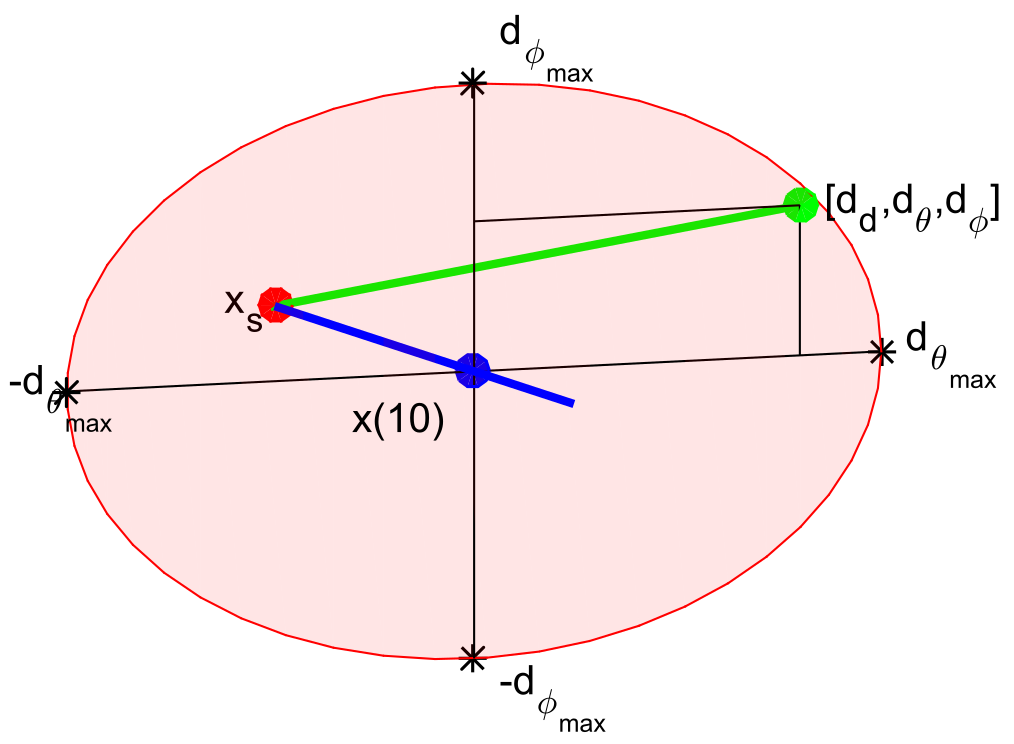
\includegraphics[width=0.7\textwidth]{\FIGDIR/TE014ElipticConeIOnePoint}         
    \caption{One rate position $[d_d,d_\theta,d_\varphi]$ (green). deviated from linear trajectory (blue line) at point ${x}(10)$.(blue) with initial position $x_s$ (red)}
    \label{fig:P21ElipticConeIOnePoint}
\end{figure}


The internal coordinate frame ${p}\in\R^2$ has origin in ${x}(t)\to\R^2$. The points of plane ${p}$ are bounded by projection ${p}=({b}-{x}(t))\to\R^2$, where $b\in D({x}(t),v)$. The point of ellipsoidal ${p}$ is then given as standard ellipse boundary with vertical span $d_\theta({x}(t))$ and horizontal span $d_\varphi({x}(t))$. 

The 2D \emph{Ellipsoid} $E({x}(t),{v})$ for specific time $t=10s$ example is portrayed  as red ellipsoid (in fig. \ref{fig:P21ElipticConeIOnePoint}).

\begin{equation}\label{eq:baseElipsoidxt}
    E({x}(t),{v})=\left\{ \begin{aligned}{b}\in\R^3:&{b}\in D({x}(t),{v}),{p}=({b}-{x}(t))\to\R^2,\\&\left(\frac{p(1)^2} {d_\theta({x}(t))^2}+ \frac{p(2)^2}{d_\varphi({x}(t))^2}\right)\le 1\end{aligned}\right\}
\end{equation}

\noindent The expected behavior of an intruder $i_k$ is to stick to predicted linear trajectory ${x}(t)$ (\ref{eq:vehiclelinearcone}). The probability of deviation should be decreasing with distance from the ellipse center (fig. \ref{fig:intruderPassingProbability}.).  


\noindent \emph{Probability density function} for ellipsoid  $E({x}(t),{v})$defined in (eq. \ref{eq:baseElipsoidxt}) is depending on maximal horizontal spread $d_\theta({x}(t))$, maximal vertical spread $d_\varphi({x}(t))$, defined by (eq. \ref{eq:elipsiodialBoudaryParameters}). 

Two standard probabilistic distributions are established $\mathscr{N}(\mu_\theta,\sigma_\theta)$ (eq. \ref{eq:elipsprobdistHorizontal}) for horizontal spread $\theta({x}(t))$ and $\mathscr{N}(\mu_\varphi,\sigma_\varphi)$  (eq. \ref{eq:elipsprobdistVertical}) for vertical spread $\varphi({x}(t))$. The means $\mu_\theta$ and $\mu_\varphi$ are set to zero, and internal coordinate frame ${p}\in\R^2$ where ${x}(t)\to\R^2$ is frame center. The variances $\sigma_\theta$ and $\sigma_\varphi$ are set as maximal distances on horizontal/vertical spread axes $d_\theta({x}(t))$ and $d_\varphi({x}(t))$.

\begin{equation}\label{eq:elipsprobdistHorizontal}
    P({x}(t),d_\theta)=\mathscr{N}(\mu_\theta,\sigma_\theta)=\mathscr{N}(0,d_\theta({x}(t)))
\end{equation}

\begin{equation}\label{eq:elipsprobdistVertical}
    P({x}(t),d_\varphi)=\mathscr{N}(\mu_\varphi,\sigma_\varphi)=\mathscr{N}(0,d_\varphi({x}(t)))
\end{equation}

\noindent The combined \emph{probability density function} for maximal spreads $d_\theta$ and $d_\varphi$ is given by (eq. \ref{eq:elipsprobdistCombined}). Because probability density function is defined for internal space ${p}\in\R^2$ and one may need to calculate impact rate for  cell space $c_{i,j,k}\in\R^3$. 

The reduction from two parameter probability distribution function to scalar rate distribution function is needed. A scalar rate distribution  function $P({x}(t),d_\theta,d_\varphi)$ over ellipsoid $E({x}(t),{v})$ is defined as (eq.\ref{eq:elipsprobdistCombined}), where the final rate is given as an average of two partial probabilities. 

Final space intersection rate $P({x}(t),d_\theta,d_\varphi)$ needs to be normalized to hold \emph{normal distribution condition} (eq. \ref{eq:normalDistrobitionCondition}). Normal distribution condition value (eq. \ref{eq:normalDistrobitionCondition}) is given as surface integral over ellipsoid $E({x}(0),{v})$ with rate distribution function $P({x}(t),d_\theta,d_\varphi)$.

\begin{equation}\label{eq:elipsprobdistCombined}
    P({x}(t),d_\theta,d_\varphi) = \frac{\mathscr{N}(\mu_\theta,\sigma_\theta)+\mathscr{N}(\mu_\varphi,\sigma_\varphi)}{2}
\end{equation}

\begin{equation}\label{eq:normalDistrobitionCondition}
    \iint_{E({x}(\tau))} P({x}(t),d_\theta,d_\varphi) \,\text{d}d_\theta\,\text{d}d_\varphi = 1
\end{equation}

\noindent Final space intersection rate  $P({x}(t),c_{i,j,k},\theta,\varphi)$  (space portion, time portion is calculated in (eq.\ref{eq:intruderIntersectionProbability}) is given by (eq. \ref{eq:spreadIntruderIntersectionProb}). Its mean value of all intersection rates $P({x}(\tau),c_{i,j,k},\theta,\varphi)$ where $\tau\in[i_e(c_{i,j,k}),i_l(c_{i,j,k})]$ is fixed point in intersection time interval.

An $P({x}(\tau),c_{i,j,k},\theta,\varphi)$ (\ref{eq:spreadIntersectionProbFixedtau}) is integration of rate density function $P({x}(\tau),d_\theta,d_\varphi)$ (eq. \ref{eq:elipsprobdistCombined}) in surface $E({x}(\tau),{v})$ to cell $c_{i,j,k}$ volume intersection. 

\begin{figure}[H]
    \centering
    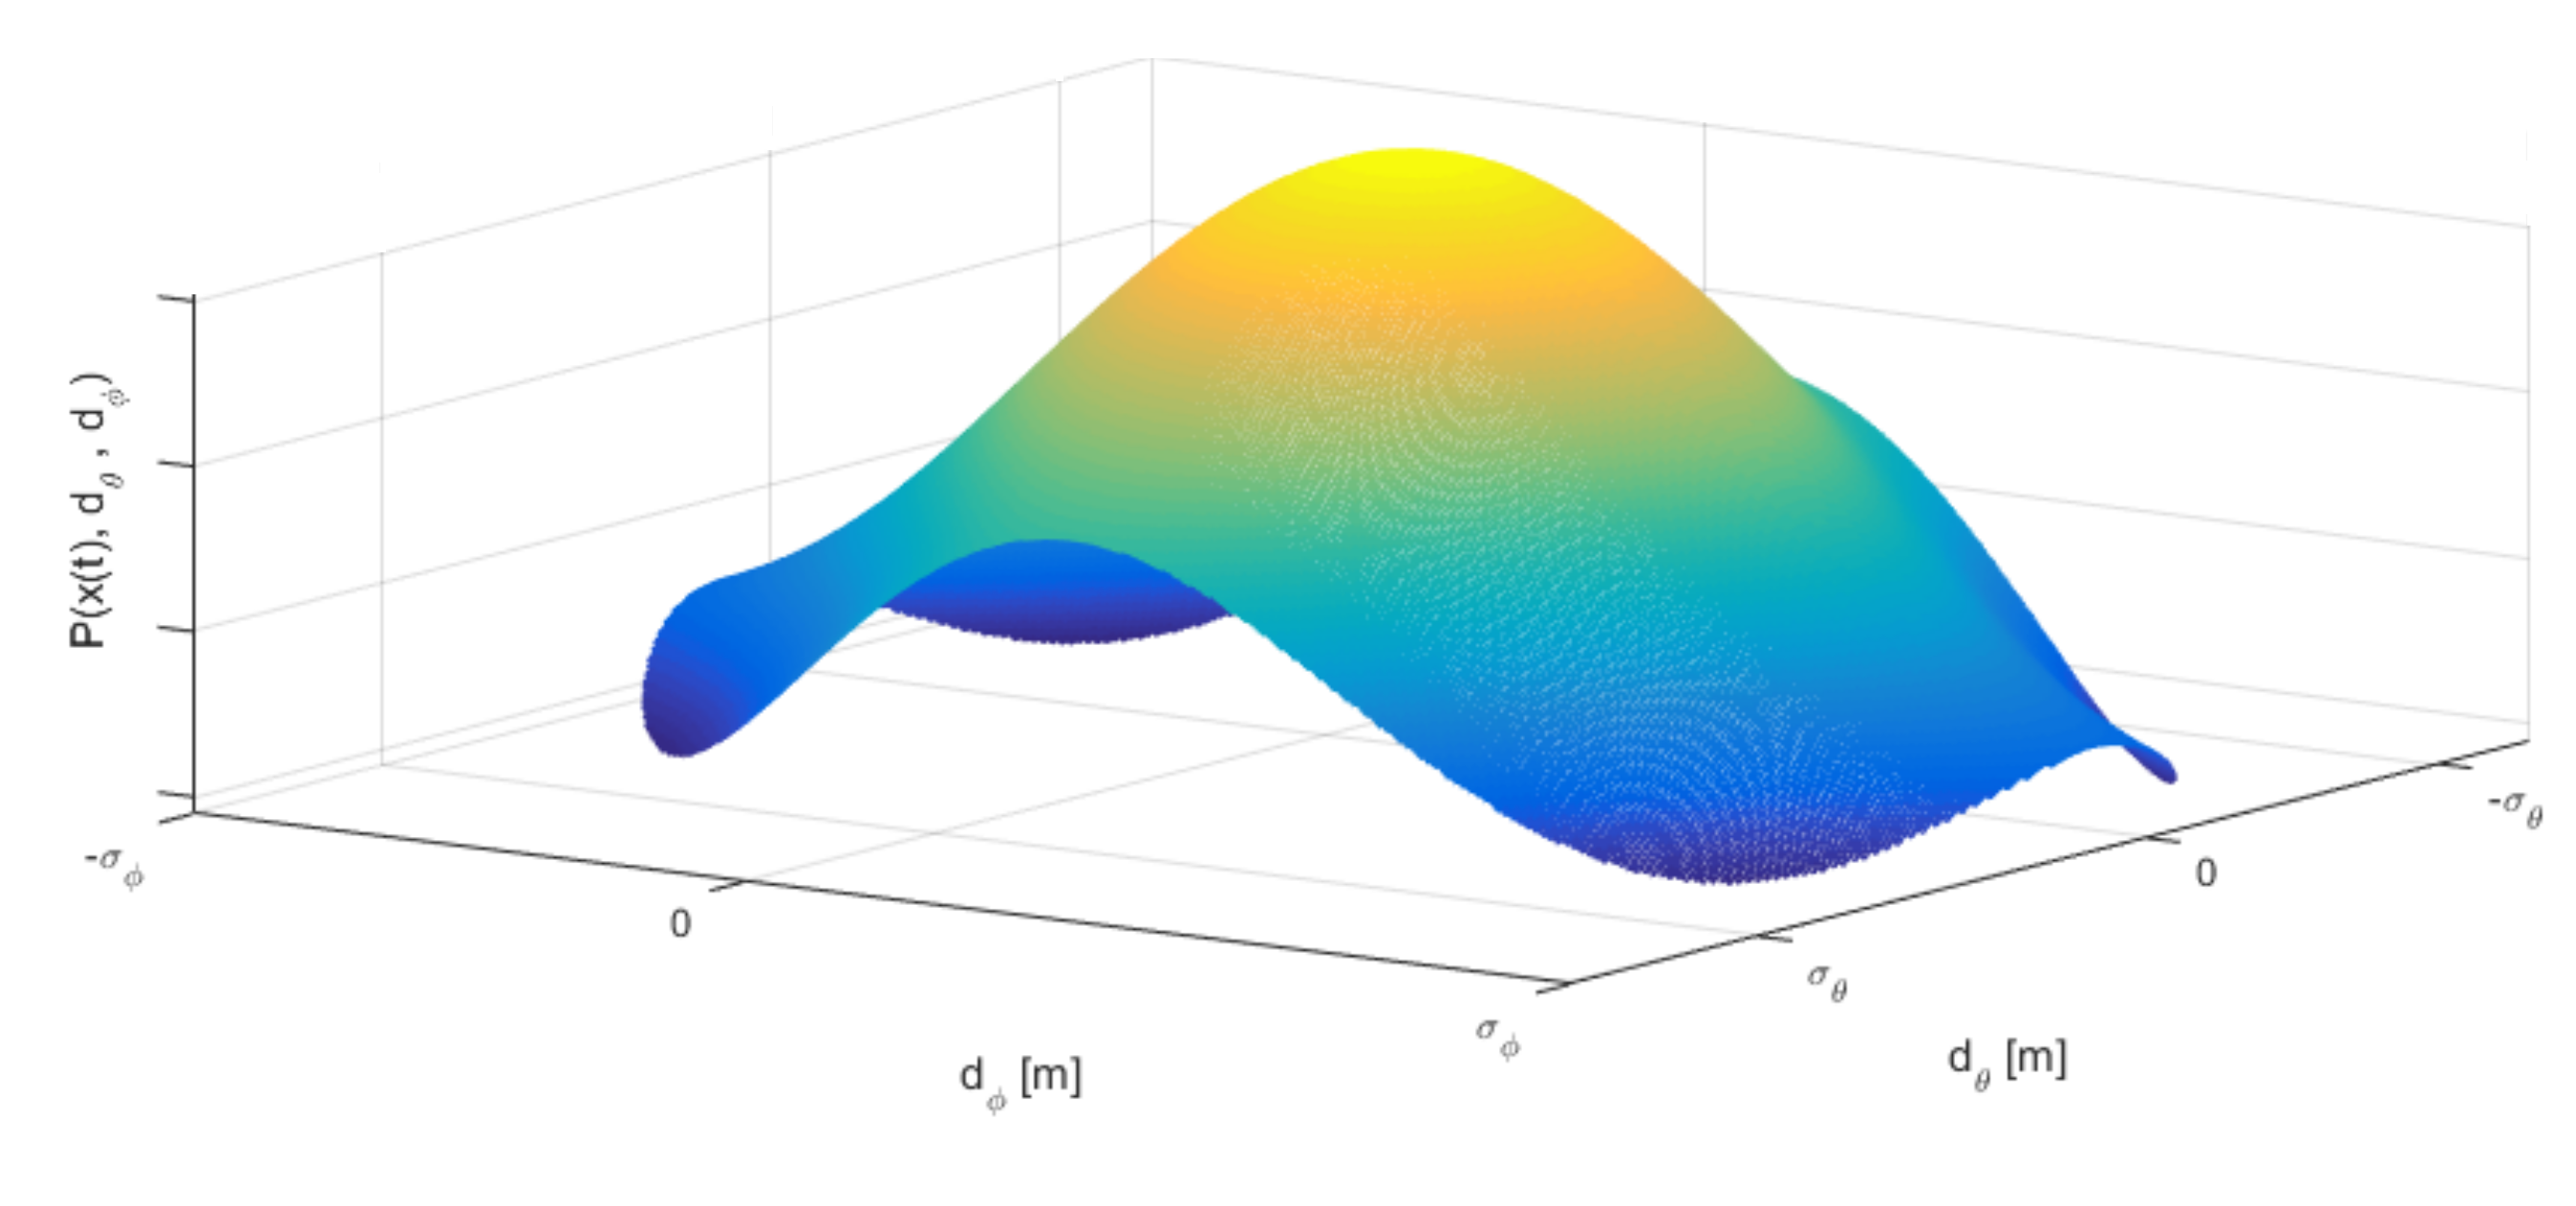
\includegraphics[width=0.9\textwidth]{\FIGDIR/TE015ProbabilisticDistributionOfEllipsoidCutSideForTE016}
    \caption{Probability of intruder $i_k$ position in ellipsoid $E({x}(t),{v})$}
    \label{fig:intruderPassingProbability}
\end{figure}

\noindent To get a volume integration partial rate in surface intersection must be integrated and normalized in time interval $\tau\in[i_e(c_{i,j,k}),i_l(c_{i,j,k})]$, the \emph{base intersection probability} $P_T(i_k({x}_s,{v},\theta,\varphi),c_{i,j,k})$ is given by (eq. \ref{eq:spreadIntruderIntersectionProb}). Example of intersection of intruder $i_r$ uncertain ellipsoid cone with avoidance grid $\mathscr{A}(t_i)$ is given in (fig. \ref{fig:ellipticConeIntersectionExample}).

\begin{equation}\label{eq:spreadIntersectionProbFixedtau}
    P({x}(\tau),c_{i,j,k},\theta,\varphi) =\iint_{E({x}(\tau),{v})\cap c_{i,j,k}} P({x}(\tau),d_\theta,d_\varphi)
\end{equation}

\begin{equation}\label{eq:spreadIntruderIntersectionProb}
    P_T(i_k({x}_s,{v},\theta,\varphi),c_{i,j,k})=\frac{\int_{i_e(c_{i,j,k})}^{i_l(c_{i,j,k})} P({x}(\tau),c_{i,j,k},\theta,\varphi)\,\text{d}\tau}{i_l(c_{i,j,k})-i_e(c_{i,j,k})}
\end{equation}

\begin{figure}[H]
    \centering
    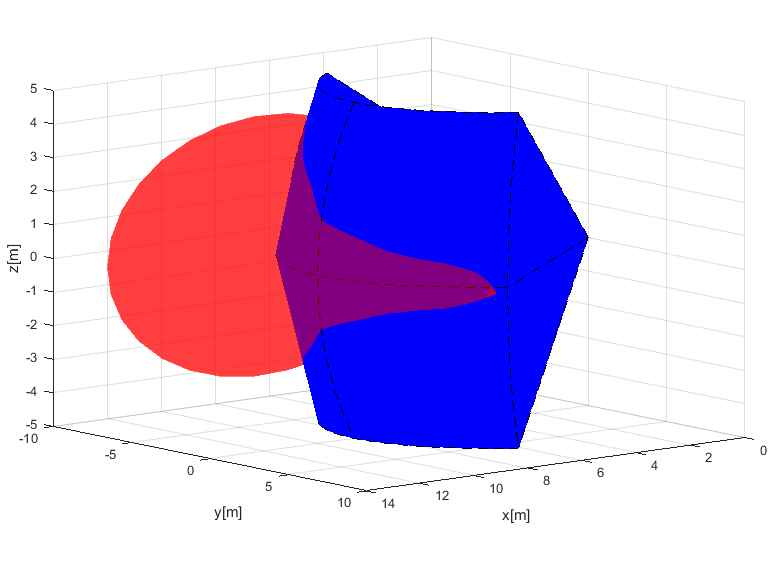
\includegraphics[width=0.7\textwidth]{\FIGDIR/TE013ElipticConeIntersecitonExample}
    \caption{Avoidance grid $\mathscr{A}(t_i)$ (blue) intersection with elliptic cone intruder $i_k({x},{v},\theta,\varphi)$ (red) example.}
    \label{fig:ellipticConeIntersectionExample}
\end{figure}

\noindent A \emph{numeric approximation} of space intersection rate $P_T(i_k({x}_s,{v},\theta,\varphi),c_{i,j,k})$ is more implementation feasible than symbolic calculation due to the multiple intersection constraints and bad intersection algorithm complexity. 

Let us define a homogeneous discrete subset of real numbers $\mathscr{R}$ which is a non-empty subset of real numbers $\R$. The set $\mathscr{R}$ (eq. \ref{eq:homogeneusdiscretizationofRealnumbers}) is homogeneous that means for an equal interval $(i,i+1],i\in\mathbb{Z}$ subset the count of members is equal to some positive natural number $k$. The parameter $k$ can be understood as \emph{unit approximation density}.

Similarly, the power sets $\mathscr{R}^2\subset\R^2$, $\mathscr{R}^3\subset\R^3$, ... $\mathscr{R}^i\subset\R^i,i\in\N^+$ keeps homogeneous distribution.

\begin{equation}\label{eq:homogeneusdiscretizationofRealnumbers}
    \mathscr{R} = \left\{\begin{aligned}a\in\R:&\forall i\in\mathbb{Z},|i<a\le i+1|=k,k\in\N^+, \\&\forall j\in \N^+a_{j+1}-a_{j}=m,m\in\R^+\end{aligned}\right\},\,\mathscr{R}\subset\mathbb{R}
\end{equation}

\noindent The orthogonal plane for ${x}(t), {v}, t \in\R$ is defined by (eq. \ref{eq:elisioidalOtrthogonalPlane}). The orthogonality property is also kept for any subspace $\mathscr{R}^n\in\R^n,n\in\N^+$. Numeric approximation of $D({x}(t),{v})$ is given as $D_D({x}(t),{v})$ (eq. \ref{eq:elisioidalOtrthogonalPlaneDiscrete}). 

The only difference is that discrete approximation is countable $|D_D|=m,m\in\N^+$, but continuous representation $|D|\approx \infty$ is uncountable. Because ellipsoid is a subset of orthogonal plane it keeps its countability property; therefore $E_D$ is also countable and must contain at least one member.

\begin{equation}\label{eq:elisioidalOtrthogonalPlaneDiscrete}
    D_D({x}(t),{v})=\left\{{a}\in\mathscr{R}^3:({a}-{x}(t))\perp{v},\right\},t\in\mathscr{R}
\end{equation}

\noindent The \emph{base ellipsoid} $E({x}(t),{v})$ for continuous-space is given by (eq. \ref{eq:baseElipsoidxt}). Every element, expect the base of internal projection $\mathscr{R}^2$ and orthogonal plane $D_D$ is same in discrete case $E_D({x}(t),{v})$ (eq. \ref{eq:baseElipsoidxtDiscrete}).

\begin{equation}\label{eq:baseElipsoidxtDiscrete}
    \bar{E}_D({x}(t),{v})=\left\{ \begin{aligned}{b}\in\mathscr{R}^3:&{b}\in D_D({x}(t),{v}),{p}=({b}-{x}(t))\to\mathscr{R}^2,\\&\left(\frac{p(1)^2} {d_\theta({x}(t))^2}+ \frac{p(2)^2}{d_\varphi({x}(t))^2}\right)\le 1\end{aligned}\right\},t\in\mathscr{R}
\end{equation}

\noindent The \emph{numeric calculation disproportion} can occur in case that ellipsoid $\bar{E}_D({x}(t),{v})$ (\ref{eq:baseElipsoidxtDiscrete}) in case of $d_\theta({x}(t))\approx 0$ and $d_\varphi({x}(t))\approx 0$. The count of ellipsoid members can be $|\bar{E}_D({x}(t),{v})|=0$, which is in contradiction with assumption $|\bar{E}_D({x}(t),{v})|\neq 0$. 

Let assume for discrete times $\tau=\left\{t_1,t_2,\dots,t_i\right\}$, $i\in \N^+$ there exists ellipsoids $\bar{E}_D({x}(t_1),{v})$,$\bar{E}_D({x}(t_1),{v})$, $\dots$, $\bar{E}_D({x}(t_i),{v})$ which are non empty and in space $\mathscr{R}^2$ in internal coordinate frame and space $\mathscr{R}^3$ in avoidance grid $\mathscr{A}(t_i)$ coordinate frame. The intersection of these partial ellipsoids in both spaces is equal to:

\begin{equation}
    \bar{E}_D({x}(t_1),{v})\cap \bar{E}_D({x}(t_2),{v})\dots\cap\dots \bar{E}_D({x}(t_i),{v}) = \varnothing
\end{equation}

\noindent An \emph{empty intersection} enables us to keep homogeneity property of ellipsoids by adding points so it is safe to add specific point ${x}(t)$ into empty ellipsoid. But only one, because it does not impact  probability density functions $\mathscr{N}(\mu_\theta,\sigma_\theta)$ and $\mathscr{N}(\mu_\varphi,\sigma_\varphi)$, neither space intersection rate  density function $P({x},d_\theta,d_\varphi)$. 

The final ellipsoid used forward $E_D({x}(t),{v})$(eq. \ref{eq:baseElipsoidxtDiscreteSafe}) is keeping all properties of ellipsoid $E({x}(t),{v})$ (eq. \ref{eq:baseElipsoidxtDiscreteSafe}). 

\begin{equation}\label{eq:baseElipsoidxtDiscreteSafe}
    E_D({x}(t),{v})= 
    \begin{cases}
        |\bar{E}_D({x}(t),{v})|=0 &: \left\{{x}(t)\right\} \\
        |\bar{E}_D({x}(t),{v})|\ge0 &: \bar{E}_D({x}(t),{v}) 
    \end{cases}
\end{equation}

\noindent The normal distribution condition for rate distribution function $P_D({x}(t),d_\theta,d_\varphi,{p})$, which is instance of to rate density function $P({x}(y),d_\theta,d_\varphi)$ (eq. \ref{eq:elipsprobdistCombined}) is used. This rate distribution must be normalized according to (eq.  \ref{eq:normalDistrobitionConditionDiscrete}).

\begin{equation}\label{eq:normalDistrobitionConditionDiscrete}
    \sum_{{p} \in E_D({x}(t))} P_D({x}(t),d_\theta,d_\varphi,{p}) = 1,\forall t\in\mathscr{R}^+
\end{equation}

\noindent The equations for \emph{space intersection rate} are similar to (eq. \ref{eq:spreadIntersectionProbFixedtau}, \ref{eq:spreadIntruderIntersectionProb}). For cell $c_{i,j,k}$ there exist intruder entry time $i_e(c_{i,j,k})$ its the earliest intersection with ellipsoid $E_D({x}(i_e(c_{i,j,k}))),{v}$. Same situation occurs with intruder leave time $i_l(c_i,j,k)$. Because $E_D$ is countable set, it means additional attributes can be attached to each point ${p}\in E_D$. Based on system dynamic (eq. \ref{eq:intruderBasicLinearModel}) the \emph{Time Of Arrival} (TOA) can be calculated. The example of TOA is given in fig. \ref{fig:intruderTimeOfArrival}.

\begin{figure}[H]
    \centering
    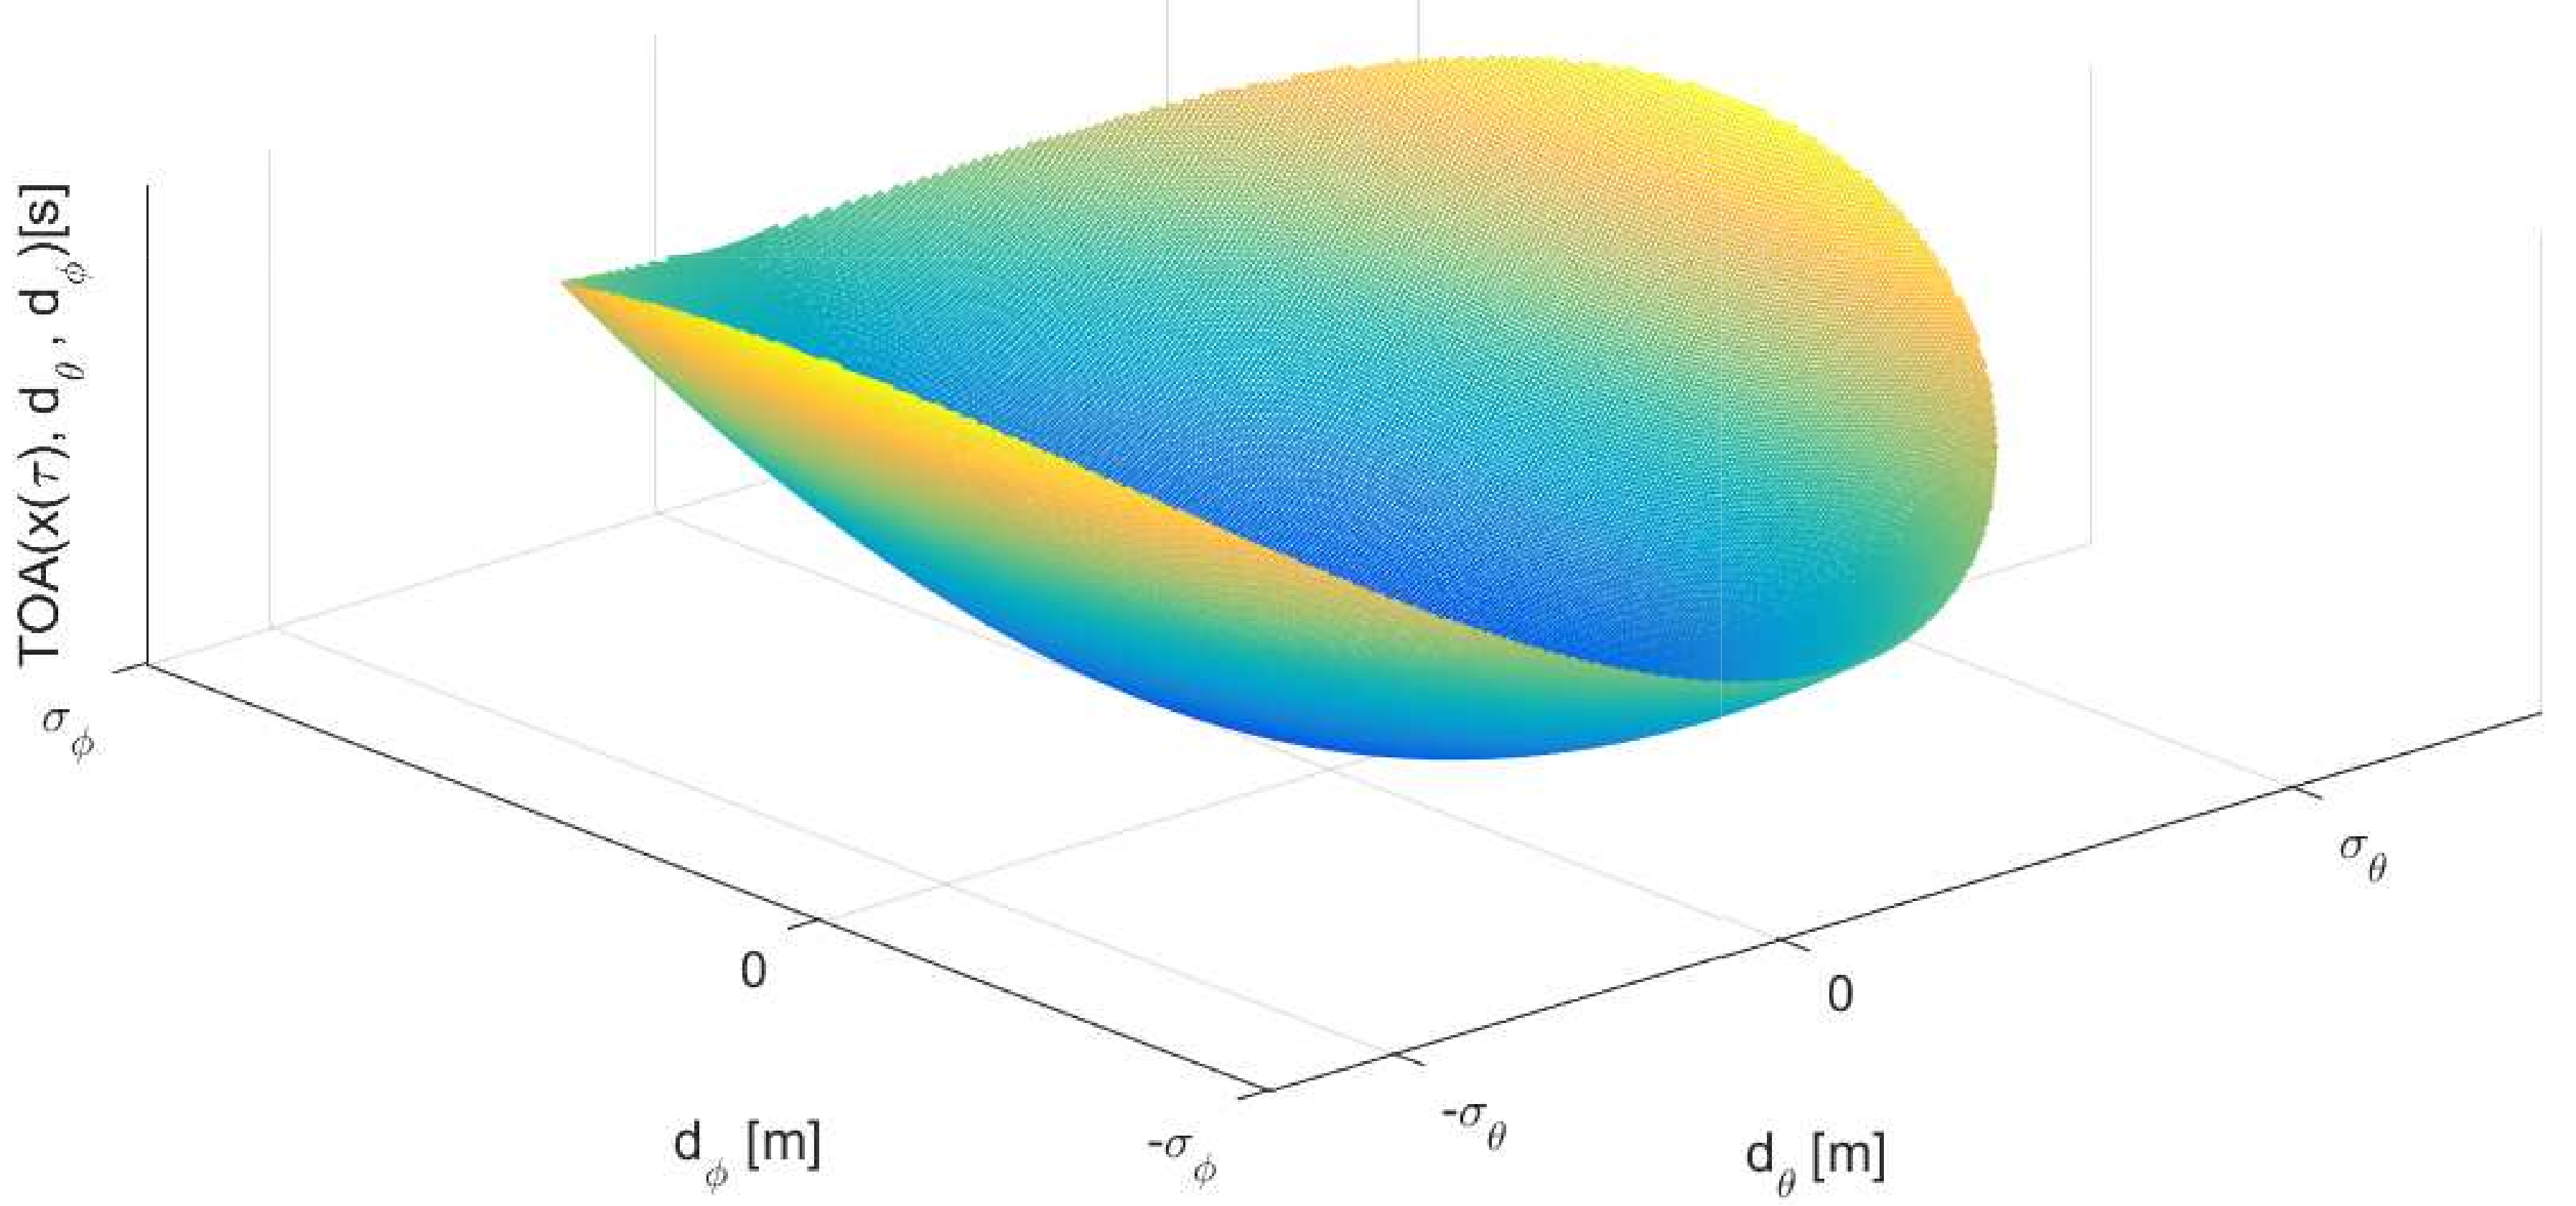
\includegraphics[width=0.7\textwidth]{\FIGDIR/TE016EllipsoidCutTimeOfArrival} 
    \caption{Time Of Arrival (TOA) for one ellipsoid $E_D({x}(\tau),{v})$.}
    \label{fig:intruderTimeOfArrival}
\end{figure}

\noindent The intersection rate $P_D({x}(\tau),c_{i,j,k},\theta,\varphi)$ for one time sample $\tau$ is given by (eq. \ref{eq:spreadIntersectionProbFixedtauDiscrete}), which has similar notation to (eq. \ref{eq:spreadIntersectionProbFixedtau}), sums are used instead of integrals and discrete rate density function $P_D({x}(\tau),d_\theta,d_\varphi,{p})$ for points form ellipse and cell intersection are used as iterator base set ${p}\in\left\{E_D({x}(\tau),{v})\cap c_{i,j,k}\right\}$.

\begin{equation}\label{eq:spreadIntersectionProbFixedtauDiscrete}
    P_D({x}(\tau),c_{i,j,k},\theta,\varphi) =\sum_{{p}\in \left\{E_D({x}(\tau),{v})\cap c_{i,j,k}\right\}} P_D({x}(\tau),d_\theta,d_\varphi,{p})
\end{equation}

\noindent The \emph{space intersection rate} $P_{TD}(i_k({x}_s,{v},\theta,\varphi),c_{i,j,k})$ (eq. \ref{eq:spreadIntruderIntersectionProbDiscrete}) is given as mean intersection rate of partial intersections $P_D({x}(\tau),c_{i,j,k},\theta,\varphi)$ where step set $T=\{$ $i_e(c_{i,j,k})$, $\dots$, $i_l(c_{i,j,k})\}$ contains all viable intersection times with ellipsoids $E({x}(\tau\in T),{v})$. The denominator is basically count of samples in sample time set $T$. 

\begin{equation}\label{eq:spreadIntruderIntersectionProbDiscrete} 
    P_{TD}(i_k({x}_s,{v},\theta,\varphi),c_{i,j,k})=\frac{\sum_{\tau=i_e(c_{i,j,k})}^{i_l(c_{i,j,k})} \sum_{{p}\in E_D({x}(\tau),{v})}P_D({x}(\tau),c_{i,j,k},\theta,\varphi,{p})}{\sum_{\tau i_l(c_{i,j,k})}^{i_e(c_{i,j,k})} 1}
\end{equation}

\noindent An \emph{intersection of intruder cone and cell} $c_{i,j,k}$ cell is defined by (eq. \ref{eq:conicIntersectionCellIntruderDiscrete}) The  set of point ${p}\in\mathscr{R}^3$ where condition of intersection between ellipsoids $E_D({x}(\tau),{v})$ for times $\tau\in\mathscr{R}^+$ and cell space $c_{i,j,k}$ is met.

\begin{equation}\label{eq:conicIntersectionCellIntruderDiscrete}
    \mathscr{P}(i_k({x}_s,{v},\theta,\varphi),c_{i,j,k})= \bigcup_{\forall \tau\in\mathscr{R}^+} \left\{{p}\in\mathscr{R}^3:{p}\in c_{i,j,k}\cap E_D({x}(\tau),{v})\right\}
\end{equation}

\noindent An \emph{intruder time of entry} $i_e(i_k,c_{i,j,k})$ (eq. \ref{eq:conicTimeOfEntryDiscrete}), for intruder $i,k$ and cell $c_{i,j,k}$ is approximated for discrete point set  $\mathscr{P}(i_k({x}_s,{v},\theta,\varphi),c_{i,j,k})$ (eq. \ref{eq:conicIntersectionCellIntruderDiscrete}) as minimal time of arrival $t_{TOA}({p})$ of member points ${p}$.

\begin{equation}\label{eq:conicTimeOfEntryDiscrete}
    i_e(i_k,c_{i,j,k})\approx \min \left\{t_{TOA}({p}):{p}\in\mathscr{P}(i_k({x}_s,{v},\theta,\varphi),c_{i,j,k})\right\}
\end{equation}

\noindent An \emph{intruder time of leave} $i_l(i_k,c_{i,j,k})$ (eq. \ref{eq:conicTimeOfLeaveDiscrete}), for intruder $i,k$ and cell $c_{i,j,k}$ is approximated for discrete point set  $\mathscr{P}(i_k({x}_s,{v},\theta,\varphi),c_{i,j,k})$ (eq. \ref{eq:conicIntersectionCellIntruderDiscrete}) as maximal time of arrival $t_{TOA}({p})$ of member points ${p}$.

\begin{equation}\label{eq:conicTimeOfLeaveDiscrete}
    i_l(i_k,c_{i,j,k})\approx \max \left\{t_{TOA}({p}):{p}\in\mathscr{P}(i_k({x}_s,{v},\theta,\varphi),c_{i,j,k})\right\}
\end{equation}

\paragraph{Combined intersection model:} The \emph{combined intersection model} $P_{O_I}(i_k,c_{i,j,k},l,b,s,\tau)$ is defined for intruder $i_k$ with parameters:

\begin{enumerate}
    \item\textit{Starting position} ${x}_s$ - expected position of intruder $i_r$ in 3D space at time of avoidance $t_i$ in avoidance grid frame $\mathscr{A}(t_i)$.
    
    \item\textit{Velocity vector} ${v}$ - oriented velocity of intruder $i_r$ at time of avoidance $t_i$ in avoidance grid frame $\mathscr{A}(t_i)$. 
    
    \item\textit{Horizontal uncertainty spread} $\theta$ - defines how much can intruder $i_r$ deviate on horizontal axis of intruder local coordinate frame (if X+ is the main axis, then Y is horizontal axis in right-hand euclidean coordinate frame), due the properties of intersection definition, the horizontal uncertainty spread can have following values $\theta\in[0,\pi/2]$.
    
    \item\textit{Vertical uncertainty spread} $\varphi$ -defines how much can intruder $i_r$ deviate on vertical axis of intruder local coordinate frame (if X+ is the main axis in local right-hand euclidean intruder coordinate frame, then Z is horizontal-vertical axis), due to the intersection definition, the vertical uncertainty spread can have following values $\varphi\in[0,\pi/2]$.
    
    \item\textit{Body volume radius} $r$ - defines the body volume of an intruder in meters and it has  $\R^+$  value.
\end{enumerate}

\noindent The \emph{flag vector} $l,b,s,\tau \in \left\{0,1\right\}$ is a parametrization  of rate calculation: $l$ stands for the \emph{lined intersection}, $b$ stands for \emph{body intersection}, $s$ stands for the \emph{spread intersection}, $\tau$ stands for \emph{time account}. 

The \emph{space intersection for line} $P_L(i_k,c_{i,j,k})$ is defined as $P_T(i_k({x},{v}),c_{i,j,k})$, where $i_k$ is intruder with properties of initial position ${x}$, velocity vector ${v}$ and $c_{i,j,k}$ is target cell. (eq. \ref{eq:baseIntersectionProbabilityLineIntersectionType}). 

The \emph{space intersection rate for body volume} $P_B(i_k,c_{i,j,k})$ is defined as $P_T(i_k({x},{v},r),c_{i,j,k})$ (eq. \ref{eq:baseIntersectionProbabilityBallIntersectionType}), where intruder $i_r$ has additional property of the intruder body volume radius $r$. 

The \emph{space intersection probability for maneuverability uncertainty} $P_S(i_k,c_{i,j,k})$ is defined as $P_{TD}(i_k({x}_s,{v},\theta,\varphi),c_{i,j,k})$ (eq. \ref{eq:spreadIntruderIntersectionProbDiscrete}), where intruder properties $\theta$, $\varphi$ stands for intruder horizontal and vertical uncertainty spread.

The \emph{time intersection rate} $P_{\tau,x}(i_k,c_{i,j,k})\in[0,1]$ is defined in (eq. \ref{eq:intruderIntersectionProbability}). This probability has two calculation modes, first is for 1D intersection (line), second is for volume intersection (body volume, spread elliptic cone).  

UAS cell entry time $t_e$ and cell leave time  $t_l$ time for a vehicle in avoidance grid $\mathscr{A}(t_i)$ is given by (eq. \ref{eq:cellEntryTime}) and (eq. \ref{eq:cellLeaveTime}). 

Intruder leave and entry time for 1D intersections is trivial and is omitted in this section. Intruder entry $i_e$ and intruder leave $i_l$ for 3D intersection is given by (eq. \ref{eq:conicTimeOfEntryDiscrete}, \ref{eq:conicTimeOfLeaveDiscrete}). 

All partial rates with respective definition references are summarized in (eq. \ref{eq:partialProbabilitiesIntruderSummary})

\begin{equation}\label{eq:partialProbabilitiesIntruderSummary}
    \begin{aligned}
        P_L(i_k,c_{i,j,k}) &= P_T(i_k({x},{v}),c_{i,j,k}) &(\ref{eq:baseIntersectionProbabilityLineIntersectionType})\\
        P_B(i_k,c_{i,j,k}) &= P_T(i_k({x},{v},r),c_{i,j,k}) &(\ref{eq:baseIntersectionProbabilityBallIntersectionType})\\
        P_S(i_k,c_{i,j,k}) &= P_{TD}(i_k({x}_s,{v},\theta,\varphi),c_{i,j,k}) &(\ref{eq:spreadIntruderIntersectionProbDiscrete})\\
        P_{\tau,x}(i_k,c_{i,j,k})&=\frac{\norm{[i_e(c_{i,j,k}),i_l(c_{i,j,k})]\cap [t_e,t_l]}}{\norm{[t_e,t_l]}}& (\ref{eq:intruderIntersectionProbability})\\
    \end{aligned}
\end{equation}

\noindent With definition of all space and time intersection rates (eq. \ref{eq:partialProbabilitiesIntruderSummary}) and given flag vector $l,b,s,\tau \in\left\{0,1\right\}$ one can formulate combined intersection rate $P_{O_I}(i_k,c_{i,j,k},l,b,s,\tau)$ (eq. \ref{eq:intruderInCellProbabilityOneIntruder}) for intruder $i_k$ and cell $c_{i,j,k}$. The principle is following: \emph{maximum of selected rates product based on flag vector is final intersection rate of intruder $i_k$ in the cell}. 

The time-use flag $\tau$ is adding time intersection rate $P_{\tau,x}(i_k,c_{i,j,k})$, where time intersection rate is defined by $x=\left\{L,B,S\right\}$ for line, body volume, spread ellipse time intersections ($P_{\tau,L}(i_k,c_{i,j,k})$ $\neq$ $P_{\tau,B}(i_k,c_{i,j,k})$ $\neq$ $P_{\tau,B}(i_k,c_{i,j,k})$ for one intruder $i_k$).

\begin{equation}\label{eq:intruderInCellProbabilityOneIntruder}
    \begin{aligned}
        P_{O_I}(i_k,c_{i,j,k},l,b,s,\tau) & = \begin{cases}\tau=0&:\max\left\{\begin{aligned}P_L(i_k,c_{i,j,k}).l\\ P_B(i_k,c_{i,j,k}).b\\P_S(i_k,c_{i,j,k}).s\end{aligned}\right\}\\\tau=1&:\max\left\{\begin{aligned}P_{\tau,L}(i_k,c_{i,j,k}).P_L(i_k,c_{i,j,k}).l\\ P_{\tau,B}(i_k,c_{i,j,k}).P_B(i_k,c_{i,j,k}).b\\P_{\tau,S}(i_k,c_{i,j,k}).P_S(i_k,c_{i,j,k}).s\end{aligned}\right\}\end{cases} &\\
    \end{aligned}
\end{equation}
		
%% This adds a line for the Bibliography in the Table of Contents.
%\addcontentsline{toc}{chapter}{Bibliography}
%% *** Set the bibliography style. ***
%% (change according to your preference/requirements)
%\bibliographystyle{plain}
%% *** Set the bibliography file. ***
%% ("thesis.bib" by default; change as needed)
\bibliography{thesis}

%% *** NOTE ***
%% If you don't use bibliography files, comment out the previous line
%% and use \begin{thebibliography}...\end{thebibliography}.  (In that
%% case, you should probably put the bibliography in a separate file and
%% `\include' or `\input' it here).

\end{document}
